\documentclass[10pt, conference, compsocconf]{IEEEtran}   	
%\usepackage{geometry}                		% See geometry.pdf to learn the layout options. There are lots.
%\geometry{letterpaper}                   		% ... or a4paper or a5paper or ... 
%\geometry{landscape}                		% Activate for for rotated page geometry
%\usepackage[parfill]{parskip}    		% Activate to begin paragraphs with an empty line rather than an indent
\usepackage{graphicx}				% Use pdf, png, jpg, or eps§ with pdflatex; use eps in DVI mode
								% TeX will automatically convert eps --> pdf in pdflatex

\usepackage{color,flushend}
\newcommand{\fix}[1]{\textcolor{black}{#1}}
\newcommand{\highlight}[1]{\textcolor{red}{#1}}
\usepackage{amssymb, amsmath}
\usepackage{mathtools}
\usepackage{booktabs}
%\usepackage[noend]{algpseudocode}
%\usepackage[ruled,vlined]{algorithm2e}
\usepackage{verbatim}
\newcommand*\rot{\rotatebox{90}}
\usepackage{clrs+} % needed for \id{} and \func{} and \call{}
%\usepackage[compatible]{algpseudocode}
\usepackage{algorithm}
\usepackage[noend]{algpseudocode}
\usepackage{varwidth}
\usepackage{multirow}
\usepackage{rotating, xcolor}
\usepackage{subfig}
\usepackage{enumitem}
%\usepackage[caption=false]{subfig}
\usepackage[hyphens]{url}
\usepackage{float}
\newfloat{algorithm}{t}{lop}

\usepackage{tcolorbox}
\definecolor{mycolor}{rgb}{0.122, 0.435, 0.698}
%\begin{tcolorbox}[width=\linewidth, boxsep=0pt, left=-4pt, boxrule=0.5pt]
%\end{tcolorbox} 
%\newtcolorbox{mybox}{colback=red!5!white,colframe=mycolor}
\makeatletter
\newcommand{\mybox}[1]{%
  %\setbox0=\hbox{#1}%
  %\setlength{\@tempdima}{\dimexpr\wd0+13pt}%
  \begin{tcolorbox}[colframe=mycolor,boxrule=0.5pt,arc=4pt,
      left=-4pt,right=6pt,top=6pt,bottom=6pt,boxsep=0pt,width=\linewidth]
    #1
  \end{tcolorbox}
}
\makeatother

\algnewcommand{\LineComment}[1]{\State \(\triangleright\) #1}
%\newcommand{\procdecl}[1]   {\proc{#1}\vrule width0pt height0pt depth 7pt \relax}
\newcommand{\lilabel}[1]        {\label{li:#1}}

\newcommand{\erdosrenyi}{Erd\H os-R\'{e}nyi }
\newcommand{\qg}{\u{g}}
\newcommand{\qG}{\u{G}}
\newcommand{\qc}{\c{c}}
\newcommand{\qC}{\c{C}}
\newcommand{\qs}{\c{s}}
\newcommand{\qS}{\c{S}}
\newcommand{\qu}{\"{u}}
\newcommand{\qU}{\"{U}}
\newcommand{\qo}{\"{o}}
\newcommand{\qO}{\"{O}}
\newcommand{\qI}{\.{I}}
\newcommand{\wa}{\^{a}}
\newcommand{\wA}{\^{A}}
\usepackage{mathtools}
\DeclarePairedDelimiter\ceil{\lceil}{\rceil}
\DeclarePairedDelimiter\floor{\lfloor}{\rfloor}


\newcommand{\minusone}{\text{-}1}

%% ABAB: Shortcuts/macros below are not used but it can be referenced as a cheatsheet
\newcommand{\liref}[1]      {line~\ref{li:#1}}
\newcommand{\Liref}[1]      {Line~\ref{li:#1}}
\newcommand{\lirefs}[2]     {lines \ref{li:#1}--\ref{li:#2}}
\newcommand{\Lirefs}[2]     {Lines \ref{li:#1}--\ref{li:#2}}
\newcommand{\lireftwo}[2]   {lines \ref{li:#1} and~\ref{li:#2}}
\newcommand{\lirefthree}[3] {lines \ref{li:#1}, \ref{li:#2}, and~\ref{li:#3}}

\def\Cpp{C{}\texttt{++}}
\newcommand{\mA}{\mathbf{A}} 
\newcommand{\mL}{\mathbf{L}}
\newcommand{\mU}{\mathbf{U}}
\newcommand{\transpose}     {^{\mbox{\scriptsize \sf T}}}
\newcommand{\mB}{\mathbf{B}}
\newcommand{\mC}{\mathbf{C}}
\newcommand{\dimN}{n}
\newcommand{\dimM}{m}
\newcommand{\dimK}{k}
\newcommand{\dnzc}{\id{nzc}}
\newcommand{\dnzr}{\id{nzr}}
\newcommand{\dni}{\id{ni}}
\newcommand{\dnnz}{\id{nnz}}
\newcommand{\dsort}{\id{sort}}
\newcommand{\dscan}{\id{scan}}
\newcommand{\dsearch}{\id{search}}
\newcommand{\dmin}{\func{min}}
\newcommand{\dmax}{\func{max}}
\newcommand{\dth}{th}
\newcommand{\dlen}{\id{len}}
\newcommand{\matlab}{{\sc Matlab}}


%\input{algobox}



\title{\LARGE LACC: A Distributed-Memory Algorithm for \\ Finding Connected Components using Matrix Algebra }


\author{Ariful~Azad,
Ayd\i n Bulu\qc~\IEEEmembership{}\\% <-this
  
  \{azad,abuluc\}@lbl.gov\\ 
  Computational Research Division \\
  Lawrence Berkeley National Laboratory \\
  %  {\small ${}^{\dagger}$ Corresponding author.}
}

\date{}	

\begin{document}
\maketitle

\section{Introduction}
Given an undirected graph $G(V, E)$ on the set of vertices $V$ and the set of edges $E$, a connected component is a subgraph in which every vertex is connected to all other vertices in the subgraph by paths and is not connected to any other vertex outside of the subgraph.  
Finding all connected components in an undirected graph is a well studied problem in graph theory with applications in bioinformatics and scientific computing. 

One particular application of connected components arises in large scale biological network clustering by Markov Clustering algorithm (MCL)~\cite{van2000graph}. 
MCL iteratively performs a series of sparse matrix manipulations to identify the clustering structure in a network. 
After the iterations converge, the clusters are extracted by finding the weakly-connected components of the final converged matrix.  This is equivalent to finding connected components on the symmetrized version of the final converged matrix, i.e., in an undirected graph represented by the converged matrix. 
In an effort to cluster large-scale networks, we have recently developed the distributed-memory parallel MCL (HipMCL)~\cite{hipmcl} algorithm.
HipMCL can cluster protein similarity networks with hundreds of billions of edges using thousands of nodes on modern supercomputers. 
Hence, we aim develop a parallel connected component algorithm that can scale to thousands of nodes. 

HipMCL is developed using linear algebraic primitives of the of Combinatorial BLAS (CombBLAS) library~\cite{bulucc2011combinatorial}. 
CombBLAS provides distributed-memory parallel primitives including sparse matrix-vector multiplication (SpMV) and sparse matrix-matrix multiplication (SpGEMM). 
CombBLAS primitives are equivalent to the recently developed GraphBLAS primitives~\cite{bulucc2017design} and can be used to develop high-performance graph algorithms quickly and efficiently. 
Hence, we primarily focus on a connected component algorithm than can be efficiently decomposed into linear algebraic primitives. 
For this reason, we selected the Awerbuch-Shiloach algorithm~\cite{awerbuch1987new} and developed a parallel decomposition of the algorithm using GraphBLAS primitives (hence the algorithm is named LACC). This algorithm is chosen for its simplicity, performance guarantees, and suitability to Combinatorial BLAS. 






\begin{figure*}[!t]
   \centering
   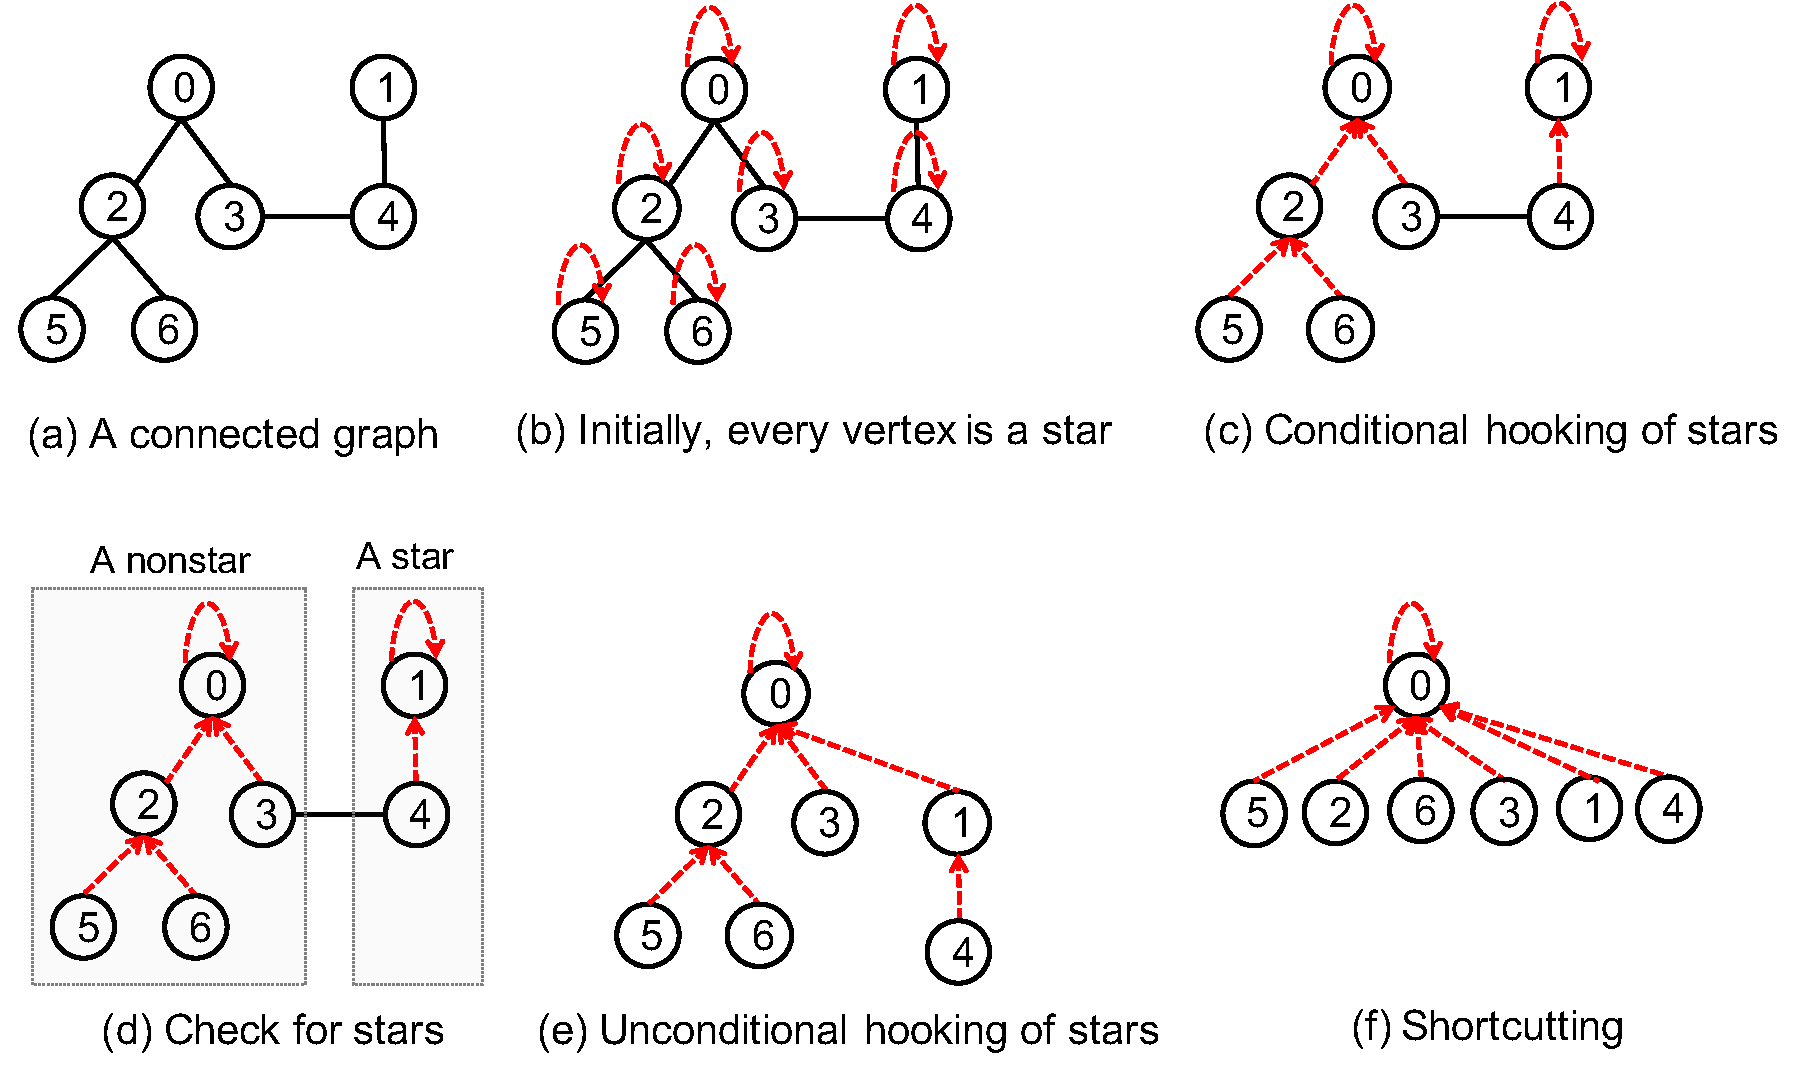
\includegraphics[scale=.45]{figures/example} 
   \caption{An illustrative example of the the Awerbuch-Shiloach algorithm. Edges in the graph are shown in solid black edges. The parent of a vertex is shown with a dashed arrowhead directed from a child to its parent. (a) An undirected and unweighted graph with seven vertices and five edges. (b) Initially, every vertex forms a singleton tree. (c) After conditional hooking of stars. Here we only show edges connected vertices in different trees. (d) Identification of vertices in stars (see Figure~\ref{fig:starcheck}). (e) After unconditional hooking of stars rooted at vertex 1. (f) After shortcutting in the only remaining tree. }
   \label{fig:example}
\end{figure*}



\begin{figure*}[!t]
   \centering
   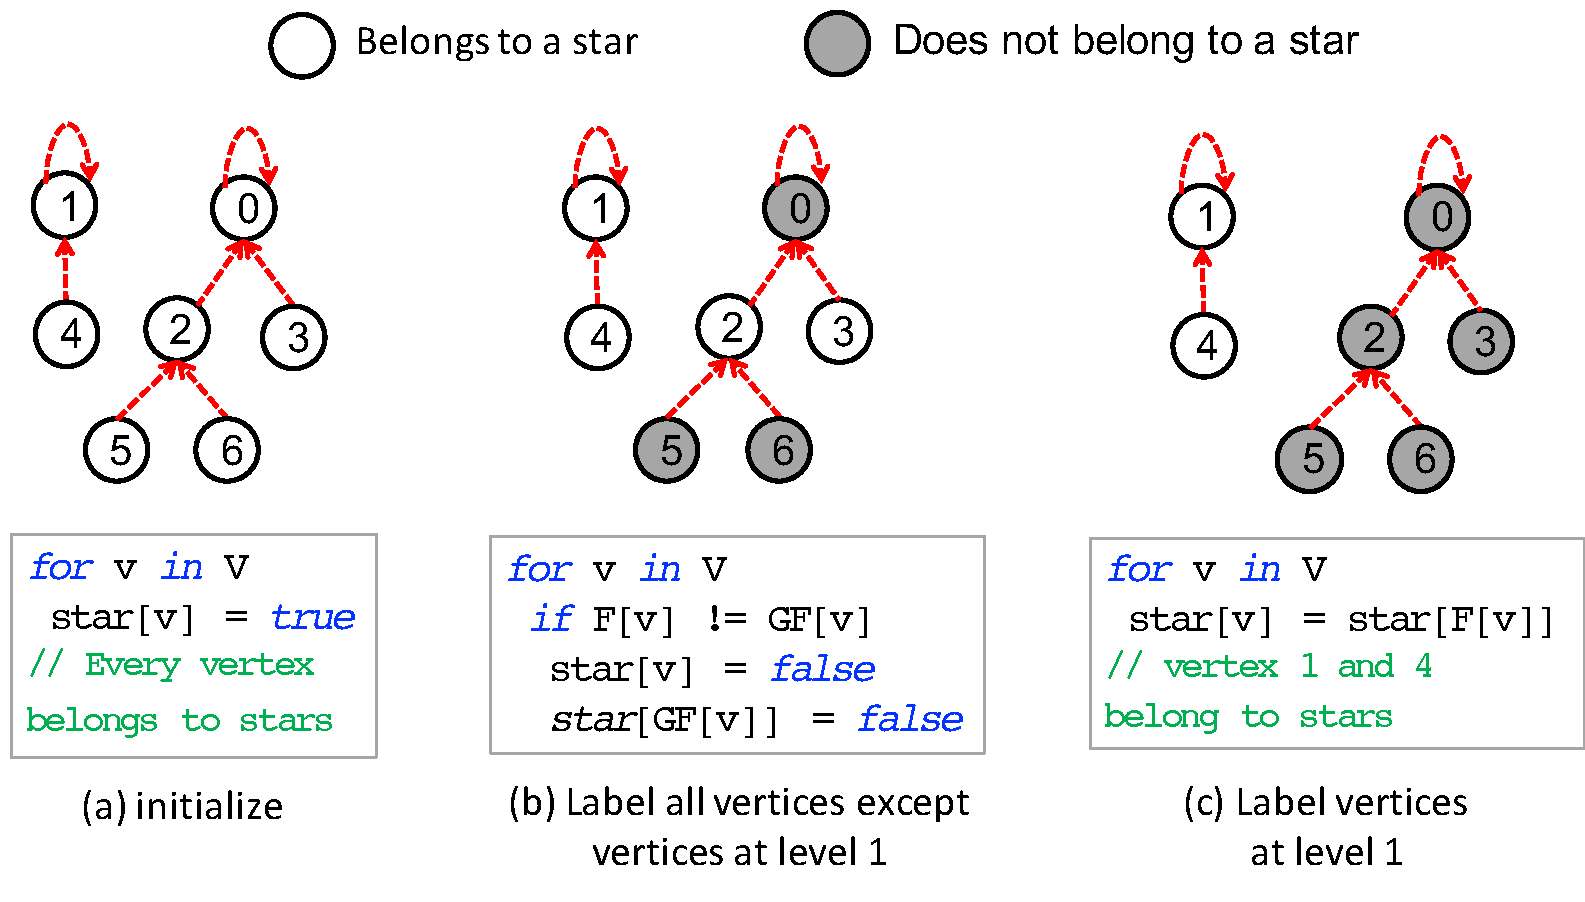
\includegraphics[scale=.45]{figures/starcheck} 
   \caption{Finding all vertices belonging stars. A Boolean array $star$ is maintained where $star[v]$ is $true$ if $v$ belongs to a star and $star[v]$ is $false$ otherwise. In this figure, a vertex belonging to a star is shown with an unfilled circle and a vertex  not belonging to a star is shown with a filled circle. The parent of a vertex is shown with a dashed arrowhead directed from a child to its parent. (a) Initially, every vertex is assumed to be part a star. (b) In a nonstar tree, we mark all vertices at level not equal to 1. (c) In a nonstar tree, we mark all vertices at level equal to 1.}
   \label{fig:starcheck}
\end{figure*}


\begin{algorithm}[!t]
\begin{algorithmic}[1]
\begin{small}
\Procedure{Awerbuch-Shiloach}{$G(V,E)$}
	\LineComment{\textcolor{blue}{Initialization }}
	\For {every vertex $v$ in $V$}
		\State $f[v] \gets u$
	\EndFor
	
	\Repeat
	\LineComment{\textcolor{blue}{Step1: Conditional star hooking }}
	\For {every edge \{$u,v$\} in $E$} {\bf in parallel }
		\If {$u$ belongs to a star and $f[u] > f[v]$}
		\State $f[f[u]] \gets f[v]$
		\EndIf
	\EndFor
	\LineComment{\textcolor{blue}{Step2: Unconditional star hooking }}
	\For {every edge \{$u,v$\} in $E$} {\bf in parallel }
		\If {$u$ belongs to a star and $f[u] \neq f[v]$}
		\State $f[f[u]] \gets f[v]$
		\EndIf

	\EndFor
	\LineComment{\textcolor{blue}{ Step3: Shortcutting}}
	\For {every vertex $v$ in $V$} {\bf in parallel }
		\State \id{gf}$[v] \gets f[f[v]]$
	\EndFor
	\For {every vertex $v$ in $V$} {\bf in parallel }
		\If {$v$ does not belongs to a star}
		\State $f[v] \gets  \id{gf}[v]]$
		\EndIf
	\EndFor
	\Until{$f$ reamins unchanged}
	\State \Return $f$
\EndProcedure
\end{small}
\end{algorithmic}
\caption{The skeleton of the Awerbuch-Shiloach algorithm. {\bf Inputs:} an undirected graph $G(V, E)$.
{\bf Output:}  An array $f$ storing the final parent of every vertex.}
\label{algo:Awerbuch-Shiloach}
\end{algorithm}


\begin{algorithm}[!t]
\begin{algorithmic}[1]
\begin{small}
\Procedure{Starcheck}{$G(V,E), f$}
	\LineComment{\textcolor{blue}{Initialization }}
	\For {every vertex $v$ in $V$} {\bf in parallel }
		\State $star[v] \gets true$
		\State \id{gf}$[v] \gets f[f[v]]$
	\EndFor
	
	\LineComment{\textcolor{blue}{Exclude vertices at depth greater than 1 and roots of nonstars }}
	\For {every vertex $v$ in $V$} {\bf in parallel }
		\If {$f[v] \neq \id{gf}[v]$}
			\State $star[v] \gets false$
			\State $star[\id{gf}[v]] \gets false$
		\EndIf
	\EndFor
	
	\LineComment{\textcolor{blue}{Exclude vertices at depth =1 in nonstar trees}}
	\For {every vertex $v$ in $V$} {\bf in parallel }
		\State $star[v] \gets star[f[v]]$
	\EndFor
	\State \Return $star$
\EndProcedure
\end{small}
\end{algorithmic}
\caption{Finding vertices belonging to stars. {\bf Inputs:} an undirected graph $G(V, E)$ and an array $f$ storing the  parent of every vertex.
{\bf Output:}  A Boolean array $star$ where $star[v]$ is $true$ if $v$ belongs to a star.}
\label{algo:Starcheck}
\end{algorithm}


\section{The Awerbuch-Shiloach algorithm}
The Awerbuch-Shiloach algorithm maintains a forest data structure where each tree represents a connected component at the current stage of the algorithm.
A tree is called a \emph{star} if every vertex is a child of the root (i.e., the height of three is at most one).
The Awerbuch-Shiloach algorithm begins with singleton trees (stars) corresponding to each vertex in the graph.
In every iteration, the algorithm merges stars with other trees (both stars and nonstars) until no such merging is possible. 
This merging is called ``hooking" in the Awerbuch-Shiloach algorithm and is performed in two steps: (a) conditional hooking and (b) unconditional hooking. These steps are described below.
Between two subsequent iterations, the algorithm reduces the hight of trees by pointer jumping, a process known as shortcutting. 
Note that the Awerbuch-Shiloach algorithm is a simplification of the Shiloach-Vishkin algorithm~\cite{shiloach1980log}. While Shiloach-Vishkin allows hooking a tree to another tree, Awerbuch-Shiloach only allows hooking a star onto another tree. Hooking stars instead of trees simplifies the hooking process and eliminate the need of some auxiliary data structures needed by the Shiloach-Vishkin algorithm.

In the Awerbuch-Shiloach algorithm, vertex $u$ maintains a parent $f[u]$ which is another vertex or itself. 
This parent-child relationship forms a directed forest where the root $u$ of a tree satisfies $f[u]=u$.
Algorithm \ref{algo:Awerbuch-Shiloach} describes the overview of the Awerbuch-Shiloach algorithm.
Initially, every vertex forms a separate star. 
In each iteration, the algorithm performs three operations: (a) conditional hooking, (b) unconditional hooking and (c) shortcutting.
Each of these three steps can be done in parallel as shown in Algorithm~\ref{algo:Awerbuch-Shiloach}.
Figure~\ref{fig:example} shows the execution of different steps of the Awerbuch-Shiloach algorithm.

Algorithm~\ref{algo:Awerbuch-Shiloach} and Figure~\ref{fig:example} assumed that the set of vertices belonging to stars is available.  
To track the star memberships, the algorithm maintains a Boolean array $star$ where $star[v]$ is $true$ if $v$ belongs to a star.
However, it is not straightforward to identify those vertices (in stars) given the parent-child relationship in the array $f$.
Figure~\ref{fig:starcheck} shows a running example of finding vertices in stars in a trees obtained from Figure~\ref{fig:example}(d).
As shown in Figure~\ref{fig:starcheck}, three steps are needed to populate the $star$ array. 
Algorithm~\ref{algo:Starcheck} describes these steps.


The Awerbuch-Shiloach algorithm terminates when every tree becomes a star and the parent array $f$ is not updated in the latest iteration. 
Awerbuch and Shiloach showed that the algorithm terminates in $O(\log n)$ iterations. Hence, using $m+n$ processors, the algorithm has $O(\log n)$ complexity in a PRAM model. 




\section{The Awerbuch-Shiloach algorithm using GraphBLAS primitives}
\label{sec:LACC}
At first, we design the Awerbuch-Shiloach algorithm in the language of sparse linear algebra.
For this purpose, we relied upon several GraphBLAS primitives as defined in its C API~\cite{bulucc2017design}.
The implementation details of these primitives (using the Combinatorial BLAS library) will be discussed in the next section.

We use three GraphBLAS operations to design the Awerbuch-Shiloach algorithm: (a) GrB\_mxv to perform sparse matrix-vector multiplication, (b) GrB\_extract for extracting some elements of a vector and (c) GrB\_assign for assigning elements of a vector to a destination vector. 
The conditional and unconditional hooking operations in the Awerbuch-Shiloach algorithm traverses the neighbors of a subset of vertices  in the graph. This operation can be captured by sparse matrix-vector (SpMV) product on an appropriate semiring.  
We refer to a semiring by listing its scaling operations, such as the (multiply, add) semiring. 
In LACC, we use Select2nd as semiring multiply, which returns the second value it is passed. 
We use min as semiring add, which returns the minimum of the two operand it is passed.
Hence, we use (Select2nd, min) semiring throughout our SpMV algorithms. 
Algorithm~\ref{algo:Sel2ndMin} describes how this semiring can be created using GraphBLAS C API.
The BFS semiring is defined
over two sets: the matrix elements are from the set of binary
numbers whereas the vector elements are from the set of
integers.

\begin{algorithm}[htbp]
\begin{algorithmic}[1]
\begin{small}
\Procedure{Semiring}{$\lvert V \rvert$}
	\State GrB\_Monoid Min
	\State GrB\_Monoid\_new(\&Min, GrB\_MIN, $\lvert V \rvert$)
	\State GrB\_Semiring Sel2ndMin
	\State GrB\_Semiring\_new(\&Sel2ndMin, Min, GrB\_SECOND)
	\State \Return Sel2ndMin
\EndProcedure
\end{small}
\end{algorithmic}
\caption{Create a semiring with (multiply, add) operations replaced by (Select2nd, min)}
\label{algo:Sel2ndMin}
\end{algorithm}



\subsection{Conditional hooking}
Algorithm~\ref{algo:condHook} describes how we designed the conditional hooking using three GraphBLAS operations.
GrB\_mxv in  Algorithm~\ref{algo:condHook} multiply the adjacency matrix $\mA$ of the graph by the parent vector $f$ on a (Select2nd, min) semiring. Since we only care about output vertices belonging to stars, we masked the output in GrB\_mxv by the Boolean vector \id{star}.
The output of GrB\_mxv is stored in $f_n$.  $f_n[v]$ stores the minimum parent of an adjacent vertex of $v$ where \id{star[v]} is true.  
Next, the GrB\_extract function extracts the parents of vertices in a star. Here we again use the \id{star} vector as an output mask.
Finally, the GrB\_assign function updates the parents of the roots of stars when possible.

\begin{algorithm}[htbp]
\begin{algorithmic}[1]
\begin{small}
\Procedure{CondHook}{$\mA$, $f$, \id{star}}
	\State Sel2ndMin $\gets$ \Call{Semiring}{$\lvert V \rvert$}
	\LineComment{\textcolor{blue}{Step1: For every vertex in a star, find a neighbor with the minimum parent id. SpMV($\mA$,  $f$) with the Sel2ndMin semiring and the output masked by \id{star} does the job. $f_n$ is the output vector. }}
	\State GrB\_mxv ($f_n$, \id{star},  GrB\_NULL,  Sel2ndMin,  $\mA$,  $f$, GrB\_NULL) \li
	\LineComment{\textcolor{blue}{Step2: Extract parents of vertices in stars ($f_{star} = f[star]$). We use GrB\_extract to extract from the parent array $f$ using \id{star} as a mask.}}
	\State GrB\_extract ($f_{star}$, \id{star},GrB\_NULL,  $f$,  GrB\_ALL, 0, GrB\_NULL) 
	\LineComment{\textcolor{blue}{Step3: Hook root of a star  to a neighboring tree ($f[f_{star}] = f_n$}).}
	\State GrB\_assign ($f$, GrB\_NULL,  GrB\_NULL,  $f_n$,  $f_{star}$,  size($f_{star}$), GrB\_NULL) 

 	%$F_n \gets$ \Call{SpMV}{$\mA, F $, SR=(select2nd, min)}  \tcp*{minimum father among all neighbors} 
	%F[V_star] = F_n[V_star]
	%GrB_extract(, star, GrB_NULL, GrB_ALL)
 \EndProcedure
\end{small}
\end{algorithmic}
\caption{Conditional hooking of stars onto other trees (both stars and non stars).  {\bf Inputs:} a sparse adjacency matrix $\mA$, a dense vector $f$ storing the parents of all vertices, a dense Boolean vector $stars$ storing whether the $i$th vertex belongs to a star.
{\bf Output:} Updated parent array $f$.}
\label{algo:condHook}
\end{algorithm}

\subsection{Unconditional hooking}
Algorithm~\ref{algo:uncondHook} describes how we designed the unconditional hooking using three GraphBLAS operations.
As shown in Algorithm~\ref{algo:Awerbuch-Shiloach},  unconditional hooking is very similar to conditional hooking  with the only different is that unconditional hooking allows a star to hook with any other tree without any restriction on the order of vertices.
However, unlike conditional hooking where a star can hook to another star or nonstar, conditional hooking enables hooking a star onto a nonstar only. 
This allows us to use a sparse vector $f_{nonstar}$ as an input to GrB\_mxv, where $f_{nonstar}$ is the subset of vertices belonging to nonstar trees. 
Hence, GrB\_mxv in  Algorithm~\ref{algo:uncondHook} multiply the adjacency matrix $\mA$ of the graph by the sparse vector $f_{nonstar}$ on a (Select2nd, min) semiring. 
In fact, (Select2nd, min) semiring is not strictly required here since the order of parents does not matter in unconditional hooking.
As before, we masked the output in GrB\_mxv by the Boolean vector \id{star}.
The output of GrB\_mxv is stored in $f_n$.  $f_n[v]$ stores the minimum parent of an adjacent vertex $w$ of $v$ where \id{star[v]} is true and \id{star[w]} is false.  
Next, the GrB\_extract function extracts the parents of vertices in a star. Here we again use the \id{star} vector as an output mask.
Finally, the GrB\_assign function updates the parents of the roots of stars when possible.


\begin{algorithm}[htbp]
\begin{algorithmic}[1]
\begin{small}
\Procedure{UncondHook}{$\mA$, $f$, \id{star}}
	\State Sel2ndMin $\gets$ \Call{Semiring}{$\lvert V \rvert$}
	\LineComment{\textcolor{blue}{Step1: Extract parents of vertices not in stars. We use GrB\_extract to extract from the parent array $f$ using the structural complement of \id{star} as a mask.}}
	\State GrB\_extract($f_{nonstar}$, \id{star},GrB\_NULL,  $f$,  GrB\_ALL, 0, GrB\_SCMP) 
	
	\LineComment{\textcolor{blue}{Step2: For every vertex in a star, find a neighbor in a nonstar. SpMV($\mA$,  $f_{nonstar}$) with the Sel2ndMin semiring and the output masked by \id{star} does the job. $f_n$ is the output vector. Min is used just to break ties. Selecting any of the two operands is sufficient here. }}
	\State GrB\_mxv ($f_n$, \id{star},  GrB\_NULL,  Sel2ndMin,  $\mA$,  $f_{nonstar}$, GrB\_NULL) 
	\LineComment{\textcolor{blue}{Step2: Extract parents of vertices in stars ($f_{star} = f[star]$). We use GrB\_extract to extract from the parent array $f$ using \id{star} as a mask.}}
	\State GrB\_extract ($f_{star}$, \id{star},GrB\_NULL,  $f$,  GrB\_ALL, 0, GrB\_NULL) 
	\LineComment{\textcolor{blue}{Step3: Hook root of a star  to a neighboring tree ($f[f_{star}] = f_n$}).}
	\State GrB\_assign ($f$, GrB\_NULL,  GrB\_NULL,  $f_n$,  $f_{star}$,  size($f_{star}$), GrB\_NULL) 

 	%$F_n \gets$ \Call{SpMV}{$\mA, F $, SR=(select2nd, min)}  \tcp*{minimum father among all neighbors} 
	%F[V_star] = F_n[V_star]
	%GrB_extract(, star, GrB_NULL, GrB_ALL)
 \EndProcedure
\end{small}
\end{algorithmic}
\caption{Unconditional hooking of stars onto other trees (only non stars).  {\bf Inputs:} a sparse adjacency matrix $\mA$, a dense vector $f$ storing the parents of all vertices, a dense Boolean vector $stars$ storing whether the $i$th vertex belongs to a star.
{\bf Output:} Updated parent array $f$.}
\label{algo:uncondHook}
\end{algorithm}


\begin{algorithm}[htbp]
\begin{algorithmic}[1]
\begin{small}
\Procedure{Shortcut}{$f$}
	\LineComment{\textcolor{blue}{Step1: find grandfathers ($\id{gf} \gets f[f] $) }}
	\State GrB\_extract (\id{gf}, GrB\_NULL, GrB\_NULL,  $f$,  $f$, 0, GrB\_NULL) 
	\LineComment{\textcolor{blue}{Step2:  $f \gets \id{gf}$}).}
	\State GrB\_assign ($f$, GrB\_NULL,  GrB\_NULL,  GrB\_ALL,  \id{gf},  size($f$), GrB\_NULL) 
 \EndProcedure
\end{small}
\end{algorithmic}
\caption{Shortcutting using GrB\_extract and GrB\_assign.  {\bf Inputs:} a dense vector $f$ storing the parents of all vertices.
{\bf Output:} Updated parent array $f$.}
\label{algo:shortcut}
\end{algorithm}


\subsection{Shortcutting}
Algorithm~\ref{algo:shortcut} describes how we designed the shortcutting using two GraphBLAS operations.
At first, we use  GrB\_extract to obtain the grand parent \id{gf} of every vertex. Next, we assign \id{gf} to the parent array by using the GrB\_assign operation.


\section{Implementing the Awerbuch-Shiloach algorithm in CombBLAS}
We use the CombBLAS framework~\cite{bulucc2011combinatorial} to implement the GraphBLAS primitives needed to implement the Awerbuch-Shiloach algorithm.
Since CombBLAS does not directly support the masking operations, we filtered out the output after performing an operation (if masking is needed). 

CombBLAS distributes its sparse matrices on a 2D $p_r \times p_c$ processor grid.
Processor $P(i,j)$ stores the submatrix $\mA_{ij}$ of dimensions $(m/p_r)\times (n/p_c)$ in its local memory. 
The CombBLAS uses the doubly compressed sparse columns (DCSC) format to store its local submatrices for scalability, 
and uses a vector of \{index, value\} pairs for storing sparse vectors. 
To balance load across processors, we randomly permute the input matrix $\mA$ before running the matching algorithms.

Vectors are also distributed on the same 2D processor grid. 
For a distributed vector $v$, the syntax $v_{ij}$ denotes the local $n/p$ length piece of the vector owned by the $P(i, j)$th processor. 
The syntax $v_i$ denotes the hypothetical $n/p_r$ or $n/p_c$ length piece of the vector collectively owned by all the processors along the $i$th processor row $P(i, :)$ or column $P(:, i)$.


\subsection{Analysis of the distributed algorithm}
We measure communication by the number of {\em words} moved ($W$) and
the number of {\em messages} sent ($S$). The cost of communicating a length $m$ message is $\alpha + \beta m$ where $\alpha$ is the
latency and $\beta$ is the inverse bandwidth, both defined relative to the cost of a single arithmetic operation. Hence, an algorithm that
performs $F$ arithmetic operations, sends $S$ messages, and moves $W$ words takes $T= F + \alpha S + \beta W$ time. 

We previously analyzed~\cite{azad2016distributed} the complexity of SpMV because it is also a building block of parallel maximal matching algorithms.
For ease of analysis, we assume that nonzeros are i.i.d. distributed in matrices and vectors. %,  $x$ is $\id{f}$ percent full, and $\mA$ has on average $d$ nonzeros per column. 
We also assume a square processor grid $p_c{=}p_r{=}\sqrt{p}$. Number of iterations is denoted by $\left\vert{\mathrm{iters}} \right\vert$.

%We leverage the 2D SpMV algorithms implemented in CombBLAS.
%The complexity of the parallel SpMSpV algorithm has been analyzed in this context recently~\cite{matchingipdps16}, hence we just state
%the result here: 
% $$ T_{ \Call{SpMV}{}}  = O \Bigl( \frac{m}{p} +  \beta  \bigl ( \frac{m}{p} + \frac{n}{\sqrt{p}} \bigr ) +  \left\vert{\mathrm{iters}} \right\vert \alpha \sqrt{p} \Bigr) .$$
 








{
\setlength{\tabcolsep}{5pt}
\begin{table}[!t]{
\centering
\begin{tabular}{rc}
					&  {\bf Cori}  \\
					& ({\bf Intel KNL}) 	\\
\hline%----------------------------------------------------------------------------
{\bf Core }	 	 & 			\\

\hline%----------------------------------------------------------------------------
Clock (GHz)			& 1.4						\\
L1 Cache (KB)		& 32					\\
L2 Cache (KB)		& 1024$^1$				\\
DP GFlop/s/core		& 44					\\
\hline%----------------------------------------------------------------------------
{\bf Node Arch.}	 	 & 			 \\
\hline%----------------------------------------------------------------------------
Sockets/node			&  1							\\
Cores per socket			& 64							\\
STREAM BW$^2$		&  102~GB/s 		\\
Memory per node		&  96~GB				\\
\hline%-------------------------------------------------------------------------
{\bf Prog. Environment}	 	 & 			 \\
\hline%----------------------------------------------------------------------------
Compiler & gcc 5.3.0 \\
Optimization & -O3  \\
\hline%----------------------------------------------------------------------------
\end{tabular}

\caption{Overview of Evaluated Platforms.  $^1$Shared between 2 cores in a tile. $^2$Memory bandwidth is measured using the STREAM copy benchmark per node.}
\label{tab:machines}
}
\end{table}
}


%\begin{table*}[!ht]
% \centering
% \caption{Test problems from the University of Florida sparse matrix collection~\cite{davis2011university}. 
%}
%
% \begin{tabular}{@{} l l c  c   c   l @{}}
%    \toprule
%    
% Class & Graph	&	\#vertices	&	\#edges &	 pseudo & Description\\
% & &	($\times 10^6$)	&	($\times 10^6$) 	&	diameter  &	\\
%
%  \toprule
%%\multirow{6}{*}{\begin{sideways}Square\end{sideways}}  
%& amazon0312	&	0.40	&	3.20			& 21	&	Amazon product co-purchasing network	\\
%& web-Google	&	0.92	&	5.11			&	16	&	Webgraph from the Google prog. contest, 2002	\\
%low-diameter graphs  &  	wikipedia-20070206	&	3.56	&		45.03	&	14	&	Wikipedia page links	\\
% & ljournal-2008	&	5.36	&		79.02 & 34	&	LiveJournal social network\\
%  &  wb-edu	&	9.85	&	57.16	&	38	&	Web crawl on .edu domain	\\
%    &  dielFilterV3real	&	1.10	&		89.31	&	84 &		High-order vector finite element method in EM\\ 	
%
%
%  \midrule 
%  &  G3\_circuit	&	1.56	&	7.66	&	514 &		circuit simulation problem	\\ 
%   &   hugetric-00020	&	7.12		&	21.36		&	3,662 &		undirected graph\\	
%  high-diameter graphs&   hugetrace-00020	&	16.00		&	48.00		&	5,633 &		Frames from 2D Dynamic Simulations\\
% &  delaunay\_n24	&	16.77		&	100.66	& 1,718	&		Delaunay triangulations of random points\\ 
%
% & rgg\_n24\_s0	&	16.77	&	165.1	&	3,069  &	Random geometric graph\\ 
%
%  	       \toprule
%  \end{tabular}
%\label{table:problem-statistics}
% \end{table*}



\section{Results}
\label{sec:results}

\subsection{Experimental Setup} 
We evaluate the performance of LACC on NERSC/Cori using the KNL processors as described in Table~\ref{tab:machines}.
We used OpenMP for multithreaded execution in our code. 
In our experiments, we only used square process grids because rectangular grids are not supported in CombBLAS~\cite{bulucc2011combinatorial}. 
When $p$ cores are allocated for an experiment, we create a $\sqrt{p/t} \times \sqrt{p/t} $ process grid where $t$ is the number of threads per process.
Unless otherwise stated, all of our experiments used 16 threads per MPI process.
In our hybrid OpenMP-MPI implementation, all MPI processes perform local computation followed by synchronized communication rounds. 
Local computation in every matrix-algebraic kernel is fully multithreaded using OpenMP.
Only one thread in every process makes MPI calls in the communication rounds (that is \texttt{MPI\_THREAD\_FUNNELED} thread support is used in \texttt{MPI\_Init\_thread} function call).
%The source code of the distributed-memory MCM algorithm is publicly available as part of Combinatorial BLAS library~\cite{CombBLAS1.5}.


 %Table~\ref{table:problem-statistics} describes a set of real matrices from the University of Florida sparse matrix collection~\cite{davis2011university} used in our experiments.
 %We selected the low-diameter scale-free graphs and high-diameter graphs arising in various scientific domains.
% To test the performance of our matching algorithm on larger matrices,  we used RMAT~\cite{rmat}, the Recursive MATrix generator to generate three different classes of synthetic matrices: (a) G500 matrices  representing graphs with skewed degree distributions from Graph 500 benchmark~\cite{graph500}, (b) SSCA matrices from HPCS Scalable Synthetic Compact Applications graph analysis (SSCA\#2) benchmark~\cite{SSCA}, and (c)  ER matrices representing \erdosrenyi~ with uniform degree distributions.
%We use the following RMAT seed parameters to generate these matrices: (a) $a{=}.57$, $b{=}c{=}.19$, and $d{=}.05$ for G500, (b) $a{=}.6$, and $b{=}c{=}d{=}.4/3$ for SSCA, and (c) $a{=}b{=}c{=}d{=}.25$ for ER.
%A scale $n$ synthetic matrix is $2^n$-by-$2^n$.
%On average, G500 and ER matrices have $32$ nonzeros, and SSCA matrices have $16$ nonzeros per row and column.
%%We compactly describe a synthetic graph, by its "scale``  where a graph has $2^{scale}$ vertices.
%For example, a scale-30 G500 matrix (\texttt{G500-30}) has about 1 billion rows, 1 billion columns, and 32 billion nonzeros.  
%We applied a random permutation to the input matrices to balance the memory and the computational load.
%%Let $A$ be an $m\times n$ matrix with $\id{nnz}$ nonzero entries.
%%We consider the matrix representing an undirected bipartite graph $G(R\cup C, E)$ where every row (column) of $A$ is represented by a vertex in $R$ ($C$), and each nonzero entry $A[i,j]$ of $A$ is represented by two edges $(r_i,c_j)$ and $(c_j,r_i)$ connecting the $i$th row and $j$th column vertices.	
%









\subsection{Impact of sorted input and output vectors on the performance of the SpMSpV-bucket algorithm}
We implemented two variants of the SpMSpV-bucket algorithm based on the sortedness of the input and output vectors: in one variant both $\mathbf{x}$ and $\mathbf{y}$ are kept sorted by their indices, while the second variant works on unsorted vectors.
Figure~\ref{fig:sorting} shows the impact of sorted vectors on the performance of the SpMSpV-bucket algorithm for $\mathbf{x}$ with 10K and 2.5M nonzeros.
When the vector is relatively dense, keeping the vectors sorted improves the performance of our algorithm as can be seen in the right subfigure in  Figure~\ref{fig:sorting}.
This is due to the fact that when $\mathbf{x}$ is denser, the probability of accessing consecutive columns of $\mA$ increases, making the bucketing step (Step 1 in Algorithm 1) more cache efficient.
By contrast, columns of  $\mA$ are often accessed inconsecutively when $\mathbf{x}$ is sparser (e.g., when $\dnnz(\mathbf{x})$ is less than $1\%$ of $n$).
Since the unsorted version never seems to outperform the sorted version in practice, we only present results with sorted vectors in the remainder of the results section.
Sorted vectors also ensure fairness when comparing our algorithm with existing algorithms (GraphMat and CombBLAS) that keep their vectors ordered. 


\begin{figure}[!t]
   \centering
   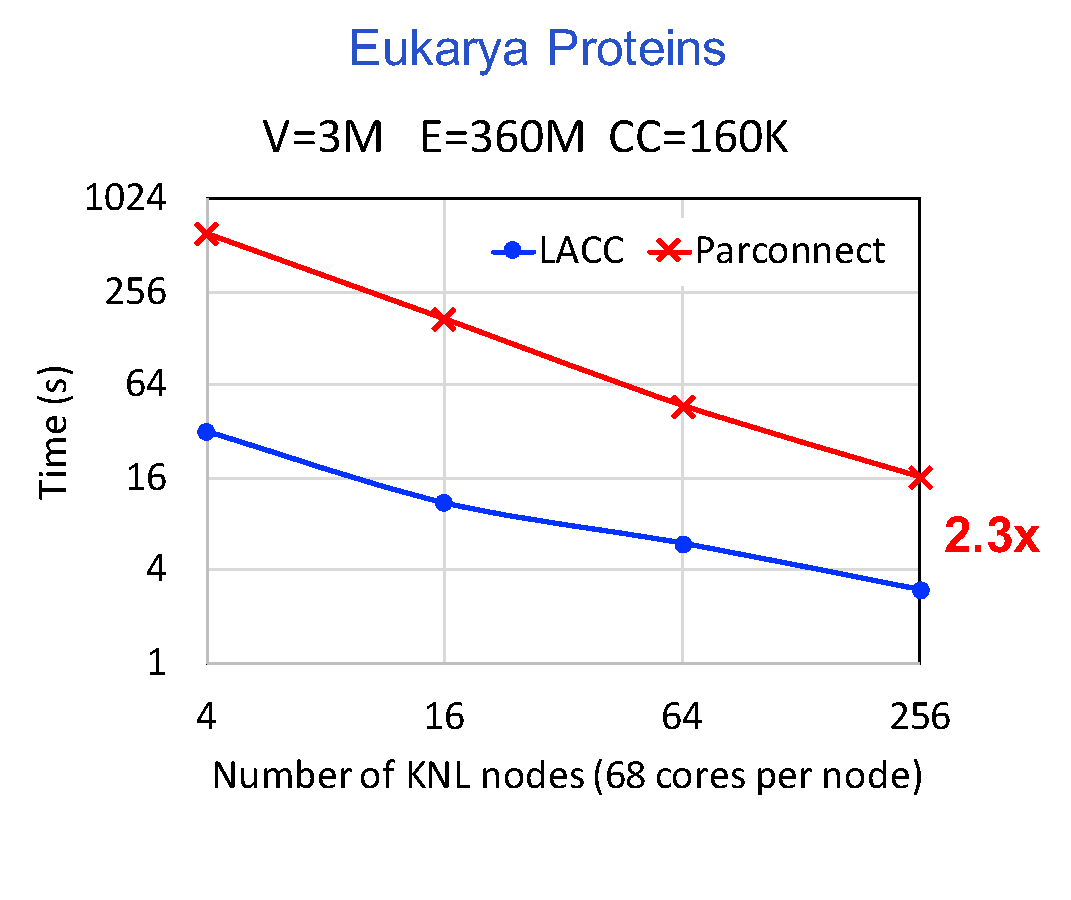
\includegraphics[scale=.5]{figures/eukarya} % requires the graphicx package
   \caption{Strong scaling of LACC and Parconnect when finding connected components in  the eukarya protein similarity network. }
   \label{fig:sorting}
\end{figure}

\begin{figure}[!t]
   \centering
   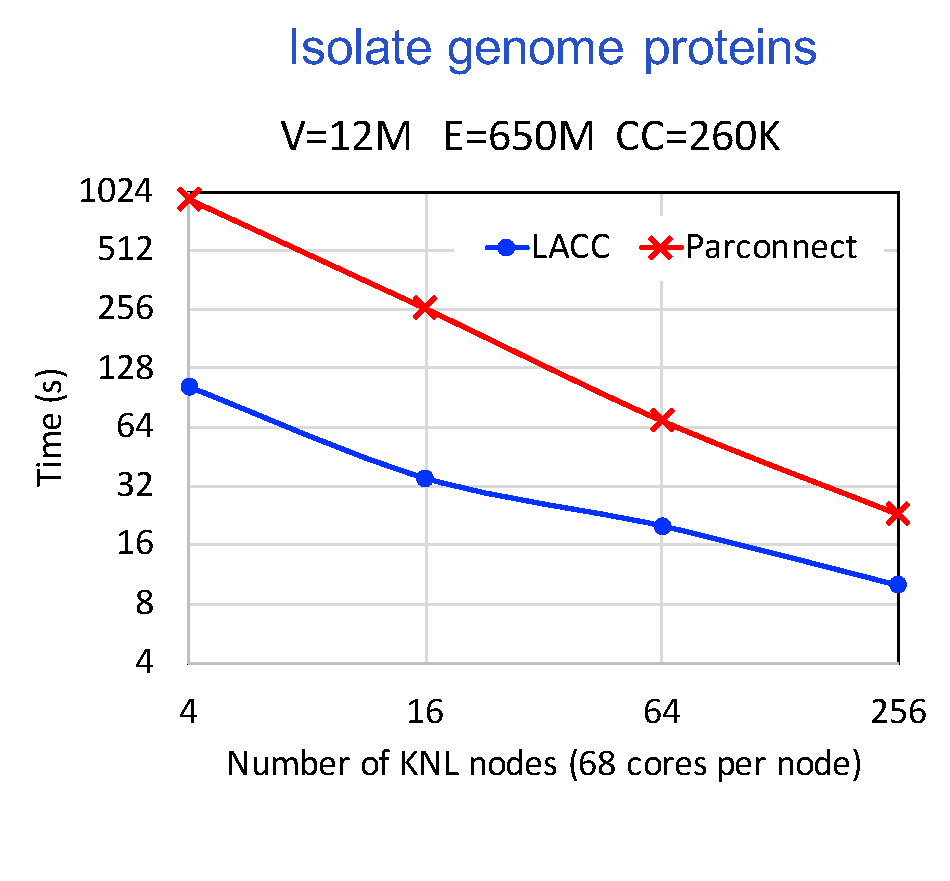
\includegraphics[scale=.5]{figures/isolates} % requires the graphicx package
   \caption{Strong scaling of LACC and Parconnect when finding connected components in  the isolate genomes protein similarity network. }
   \label{fig:multiply_nnzx}
\end{figure}





%\input{augmentation}





%\subsection{}


\bibliographystyle{IEEEtran}
\bibliography{LACC}


\end{document}  